
\chapter{Channels and State}
\label{chap:channels:state}

Suppose that we are developing a protocol.  We may well want to work
out the overall message flow, and understand the consequences of
different choices, before we figure out how---concretely---to protect
particular messages.  For instance, we may know that the sender of a
particular message will want to ensure that its contents will remain
confidential, without selecting a particular mechanism for doing so.
Having worked out the overall structure of the protocol, it may later
be clear how to discharge the assumption that the contents remain
confidential.  Or in other cases, we may know that we will use the
same main message flow in several contexts, and in each of those
contexts there may be different mechanisms that would make sense.

In those kinds of development, {\cpsa} allows us to assume that
messages are transmitted over \emph{channels} that are assumed to
offer security guarantees to the messages they carry.  The treatment
of channels also helped determine an approach to representing
long-term, cross-session mutable state in {\cpsa}.  The goal of this
chapter is to explain how to use the {\cpsa} channel mechanism, and to
build on that understanding to work with long-term mutable state.  

\paragraph{Channel security guarantees.}  The most important
guarantees are \emph{authenticated} channels and \emph{confidential}
channels.  They stipulate actions that must be taken by some instance
of a role of the protocol, rather than by the adversary.
%
\begin{itemize}
  \item An authenticated channel guarantees to the recipient of a
  message that this message was sent by some instance of a role of the
  protocol.
  \item A confidential channel guarantees to the sender that this
  transmission will not be received by the adversary, i.e.~that any
  recipient is an instance of a role of the protocol.  Hence, any
  disclosure of not-yet-public parts of the message occur only if the
  message is received and acted on by one or more instances of
  protocol roles.
\end{itemize}
%
A channel that is both \emph{authenticated} and \emph{confidential} is
sometimes called a \emph{secure} channel.

Later, when we have developed an adequate protocol using the channel
properties, we can refine it to one or more protocols that use
specific cryptographic mechanisms to achieve the properties we need.
For instance, digital signatures or Message Authentication Codes can
achieve authenticity, public-key encryption can achieve
confidentiality, and symmetric encryption (e.g.~an authenticated
encryption mode) can implement a secure channel.

Likewise, specific TLS modes can be used to implement authentic,
confidential, and secure channels.  For instance, a typical
unilaterally authenticated TLS connection provides the client an
authenticated channel for messages from the server, while it provides
a confidential channel for messages to the server.  In itself, the TLS
unilateral handshake provides no guarantee to the server.

Other properties of channels are sometimes of interest, but are not
directly implemented by {\cpsa}.  For instance, a \emph{fair} channel
ensures that a message transmitted onto it will eventually be
delivered to some instance of a role of the protocol.  A
\emph{deliver-once} channel ensures that a message transmitted onto it
will be delivered at most once to any instance of a role of the
protocol.  \emph{In-order delivery} is another possible channel
property.  Some of these may be represented indirectly in {\cpsa}
specifications~\cite{Guttman12}.  However, authenticated and
confidential channels are often useful in protocol design, and fit
smoothly into the {\cpsa} authentication test method.

In Section~\ref{sec:channels:state:ch}, we describe how to use the
{\cpsa} channel mechanism.

\paragraph{Channels and long-term state.}  In
Section~\ref{sec:channels:state:state}, we also describe a model of
protocols that rely on long-term, cross-session state, which is based
on the channel mechanism.  Here we consider a regular principal that
interacts privately with a device containing some registers that
maintain state.\footnote{By a \emph{regular} principal for a protocol
  $\Pi$, we mean a non-adversarial principal, i.e.~one that acts only
  in accordance with the protocol $\Pi$.}
%
The principal may read values out of the state registers and write
back other values, often related values; these actions determine the
state transitions the device can undergo when used in this protocol.

The connection with channels is this.  When a regular protocol
participant writes a value into a state register, this is akin to
sending a message to oneself at a future moment.  What one relies on,
when using this mechanism, is that the recipient of this
message---one's future self---is still a regular participant, so that
any future disclosure to the adversary will be due to some other
action.  That is, writing to a state register is sending a message on
a confidential channel.

When reading from a state register, there are two possibilities.  One
is that one's past self wrote this value into the state register
previously.  In this case, reading from the state register is like
receiving a message on an authenticated channel.  However, there is
another case also, in which the value read may simply have been an
initial state, available from the state register at power-up, so to
speak.  We call a state value a \emph{generated state value} when the
second case cannot apply to it, i.e.~it is a value that may have been
written into the register but was definitely not available simply as
an initial, power-up value.  We summarize the idea by saying that
reading a generated state value from a state register is receiving a
authenticated value from a channel.

Thus, state registers offer a confidentiality property for written
values, and an authenticity property for read values, if they are
generated values.  Thus, for state registers, the duality of
confidentiality and authenticity holds in a limited form, i.e.~for
generated values.  This is the reason why {\cpsa} implements state via
the same ideas as confidential and authenticated channels, although
state requires some additional properties that will be described below
in Section~\ref{sec:channels:state:state}.   

\section{Channels}
\label{sec:channels:state:ch}

The {\cpsa} model of authenticated or confidential channels requires
only a small amount of syntax.  First, variables of sort \verb|chan|
may be declared to range over channels, for instance:
%
\begin{verbatim}
    (vars ... (ch-name-1 ch-name-2 chan) ...)
\end{verbatim}
%
Second, a transmission event or reception event may have an additional
component that is a variable of sort \verb|chan|, taking the forms:  
%
\begin{verbatim}
    (send ch-name-1 sent-msg)
    (recv ch-name-2 recvd-msg) 
\end{verbatim}
%
Finally, we may assert the \emph{authenticated} or \emph{confidential}
property of a channel, using the annotations:
%
\begin{verbatim}
    (auth ch-name-1 ch-name-2)
    (conf ch-name-2) 
\end{verbatim}
%
As with annotations such as \verb|uniq-orig| and \verb|non-orig|,
these can appear either within a \verb|defskeleton| query form or
within a \verb|defrole| role declaration.  As in the previous cases,
the semantics for an annotation in a particular query is that the
annotation holds only for that specific instance.  An annotation in a
role declaration is a much stronger assumption.  It instructs {\cpsa}
to add the instance of the assumption \emph{every time} it adds an
instance of that role.  Since it is a much stronger assumption, it
yields less precise analyses.

\subsection{Yahalom with Channels}
\label{sec:channels:state:ch:yahalom}

We provide two examples of the channel mechanism, both based on the
Yahalom protocol.  They both use channels with annotations to explain
the security properties needed for interaction with the key server.
An explicit encryption is present only for the last message, in which
the initiator encrypts and returns the responder's nonce, establishing
that the session key has been received and accepted, and was indeed
requested by the initiator when starting the session.

In the first version (Section~\ref{sec:channels:state:ch:role:level}),
we ``take the easy way out,'' and incorporate the channel annotations
into the role definitions, meaning that {\cpsa} will introduce a new
instance of the assumption for every instance of a role that it
considers.

In the second version, we use the slower mechanism, and introduce each
individual channel property in a declaration in the \verb|defskeleton|
query forms.  From the latter we learn a kind of
\emph{session-independence\/}:  The security properties of a
particular session of the protocol depend only in the channels that
should be used in that protocol session, and the messages cannot leak
from one session to undermine the security goals of another session.

It is perfectly reasonable in a development process to explore the
protocol design choices with the channel annotations as assumptions at
the role definition level first.  When analysis shows that a version
is acceptable, then one can remove the role definition annotations,
and add assumptions strand-by-strand during a stepwise analysis.

If this analysis yields an acceptable result, for instance the
session-independence property, one can then further refine the
protocol by incorporating cryptographic mechanisms to ensure the
channel properties are met.  In the original Yahalom protocol (see
e.g.~\cite{Paulson97c}), the channels are implemented via symmetric
cryptography.  If the initiator and responder each share an
uncompromised long term key with the server, then an authenticated
encryption mode certainly satisfies the channel properties.  However,
other mechanisms are also possible, e.g.~asymmetric primitives or,
indeed, TLS.

Indeed, a choice of a particular primitive early in the design process
obscures what actual properties are needed for the protocol to achieve
its goals.


\paragraph{Yahalom:  Protocol idea.}  In the Yahalom protocol, the
initiator $A$ provides a nonce $N_A$ to the responder $B$, who passes
that along with its own nonce $N_B$ and both names $A,B$ to a key
server.  The server then creates a fresh session key $K$ for $A$ and
$B$, packaging it separately for $A$ and for $B$ with their names; the
package for $A$ also contains $N_A,N_B$.  $A$ completes the exchange
by encrypting $B$'s nonce $N_B$ with the session key $K$.

\paragraph{Yahalom:  Channel assumptions.}  In any session, the server
needs a confidentiality guarantee for the packages it sends in order
to protect the session key $K$ in that session.  So that requires the
channel confidentiality property for the outbound channels from the
server.  Moreover, the initiator and responder each need an
authentication guarantee for the packages it receives, so as to know
that the key is safe to use.

\subsection{Yahalom with Channels, 1:  Role-level assumptions}
\label{sec:channels:state:ch:role:level}

We first codify the confidentiality and authenticity channel
properties using annotations in the role declarations.  This
corresponds to the stronger assumption that compliant principals
\emph{always} use channels that successfully achieve those security
properties.  Since the assumption is stronger, any conclusions we
reach will be \emph{weaker} conclusions: they are implications that
depend on a stronger hypothesis.  In
Section~\ref{sec:channels:state:ch:strand:level}, we will show how,
with a bit of extra work, we can find the tightest relevant
hypotheses.

In Fig.~\ref{fig:yahalom:ch:role} we show the three roles of the
protocol with the behavior and channel assumptions mentioned at the
end of Section~\ref{sec:channels:state:ch:yahalom}.  {\cpsa} will
automatically instantiate the channel assumptions for each role every
time it incorporates an instance of the role.   
%
\begin{figure}\small
%
\begin{verbatim}(defprotocol yahalom basic
  (defrole init
    (vars (a b c name) (n-a n-b text) (k skey) (ch3 chan))
    (trace (send (cat a n-a))
           (recv ch3 (cat a b k n-a n-b))
           (send (enc n-b k)))
    (auth ch3))

  (defrole resp
    (vars (b a c name) (n-a n-b text) (k skey) (ch1 ch2 chan))
    (trace (recv (cat a n-a))
           (send ch1 (cat a b n-a n-b))
           (recv ch2 (cat a b k))
           (recv (enc n-b k)))
    (auth ch2))

  (defrole serv
    (vars (c a b name) (n-a n-b text) (k skey) (ch1 ch2 ch3 chan))
    (trace (recv ch1 (cat a b n-a n-b))
           (send ch3 (cat a b k n-a n-b))
           (send ch2 (cat a b k)))
    (conf ch3 ch2)
    (uniq-orig k)))\end{verbatim}
  \caption[Yahalom (role decls.)]{Yahalom protocol with channel
    assumptions in role declarations}
  \label{fig:yahalom:ch:role}
\end{figure}

We can now ask {\cpsa} a succession of queries about this protocol.
First, if the responder has a complete, four-step local session, then
there are corresponding server and initiator runs
(Fig.~\ref{fig:yahalom:ch:resp:pov}).  All participants agree on the
identities $A,B$, the responder's nonce $N_b$, and the session key
$K$.  Moreover, the server and initiator agree on the initiator's
nonce $N_A$, but the responder does not need to.
%
\begin{figure}
  \centering
  \begin{minipage}[c][2.5in][c]{.4\linewidth}
    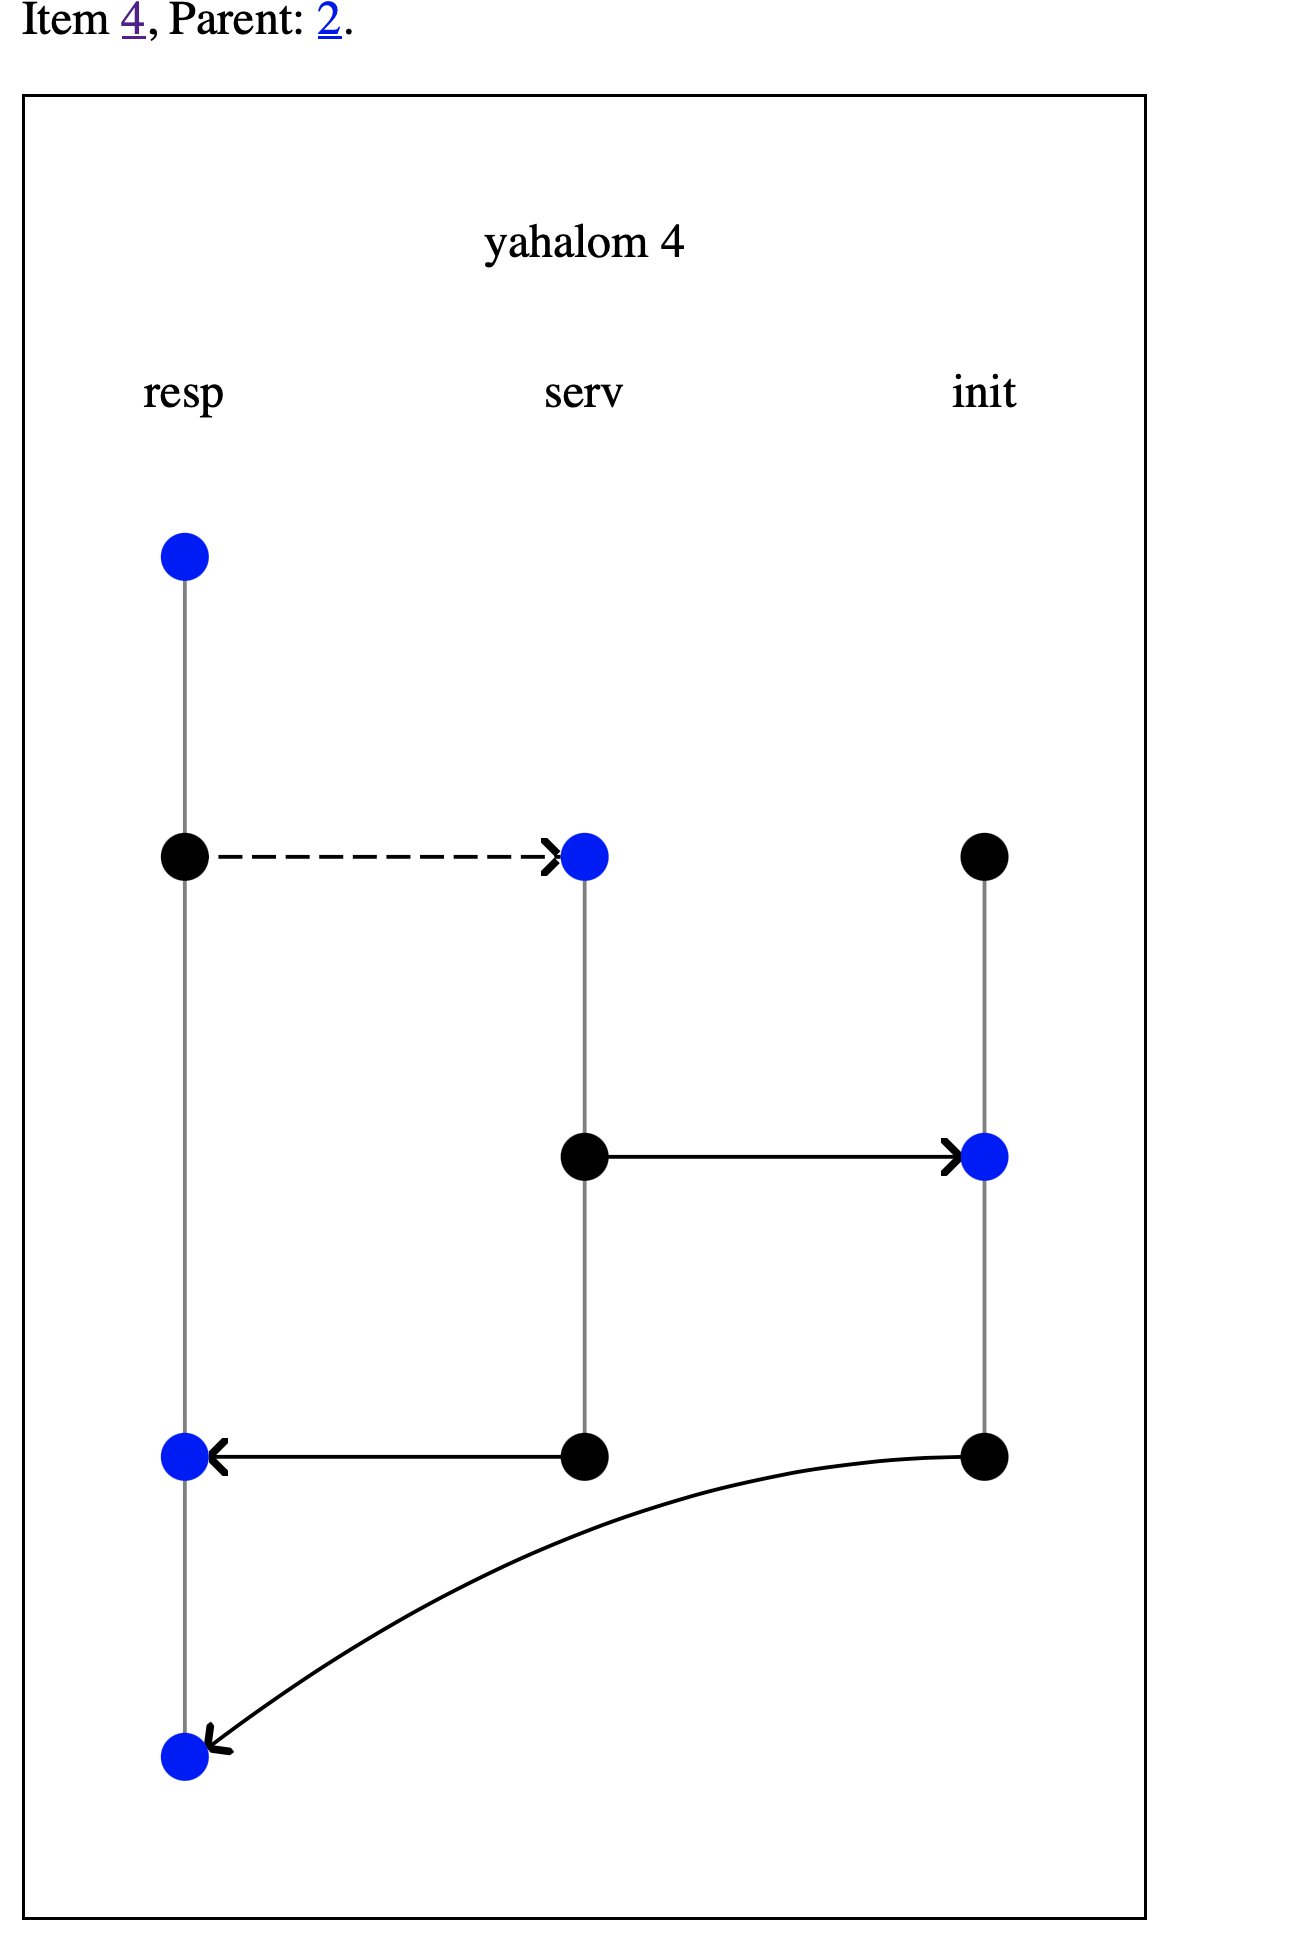
\includegraphics[height=2.5in]{yahalom_ch_resp_pov.png} 
  \end{minipage}
  \begin{minipage}[c][2.5in][c]{.5\linewidth}\small
\begin{verbatim}(defstrand resp 4 (k k) (n-a n-a)
           (n-b n-b) (b b) (a a) ...)

(defstrand serv 3 (k k) (n-a n-a-0)
           (n-b n-b) (a a) (b b) ...)

(defstrand init 3 (k k) (n-a n-a-0)
           (n-b n-b) (a a) (b b) ...)
\end{verbatim}
  \end{minipage}
  \caption{The responder's point of view}
  \label{fig:yahalom:ch:resp:pov}
\end{figure}
%
{\cpsa} also validates that the session key $K$ cannot be disclosed.

When we ask what follows if the initiator has a full local session,
the result is more limited.  The initiator authenticates a server
session of at least length two, agreeing on the identities $A,B$, the
two nonces, and the session key $K$.  Again, {\cpsa} validates that
$K$ cannot be disclosed.

Observe that if any initiator and responder have local sessions
involving a shared key $K$, then at least the result of
Fig.~\ref{fig:yahalom:ch:resp:pov} must hold, and they agree on each
other's identities $A,B$.

The server receives no authentication guarantees from the protocol as
defined here, but is guaranteed that the shared key $K$ will remain
undisclosed.  This is undesirable from one point of view, as it may
cost resources for the key server to generate a new key and package
it.  Thus, an adversary can force this to occur as desired.  This is
(presumably) the reason why the original Yahalom protocol encrypts the
message from the responder to the server (the arrow that appears
dashed in Fig.~\ref{fig:yahalom:ch:resp:pov}).  We may achieve the
desired effect by stipulating that the server's channel \verb|ch1| is
authenticated.  Our analysis shows that there is no benefit to
confidentiality on that channel.

One might, however, doubt whether there is much benefit to the
\texttt{(auth ch1)} stipulation, since the adversary can still arrange
for messages from legitimate responders to be delivered repeatedly.

We can infer from this analysis that symmetric authenticated
encryption long term key shared between the key server and each client
is a good way to implement the channels \verb|ch2| and \verb|ch3|,
since the key server relies on their confidentiality property and the
clients rely on their authentication property.  


\subsection{Yahalom with Channels, 2:  Per-strand assumptions}
\label{sec:channels:state:ch:strand:level}

We now remove the role definition annotations, i.e.~we omit the
\texttt{(conf ch3 ch2)} annotation from the declaration of the server,
and we omit the \texttt{(auth ch2)} and \texttt{(auth ch3)}
annotations from the responder and initiator declarations, resp.  We
will now ask a succession of queries, each eliciting some more
information, and allowing us to add small assumptions at each stage to
identify the individual channel properties that matter.  First, we
ask:
%
{\small
\begin{verbatim}(defskeleton yahalom
  (vars (a b c name) (n-b text) (ch1 ch2 chan))
  (defstrand resp 4 (a a) (b b) (n-b n-b) (ch1 ch1) (ch2 ch2))
  (auth ch2)   
  (uniq-orig n-b))\end{verbatim}}
%
This yields the output in Fig.~\ref{fig:yahalom:q:resp:pov:1}.
%
\begin{figure}
  \begin{minipage}[c][2in][c]{.25\linewidth}
    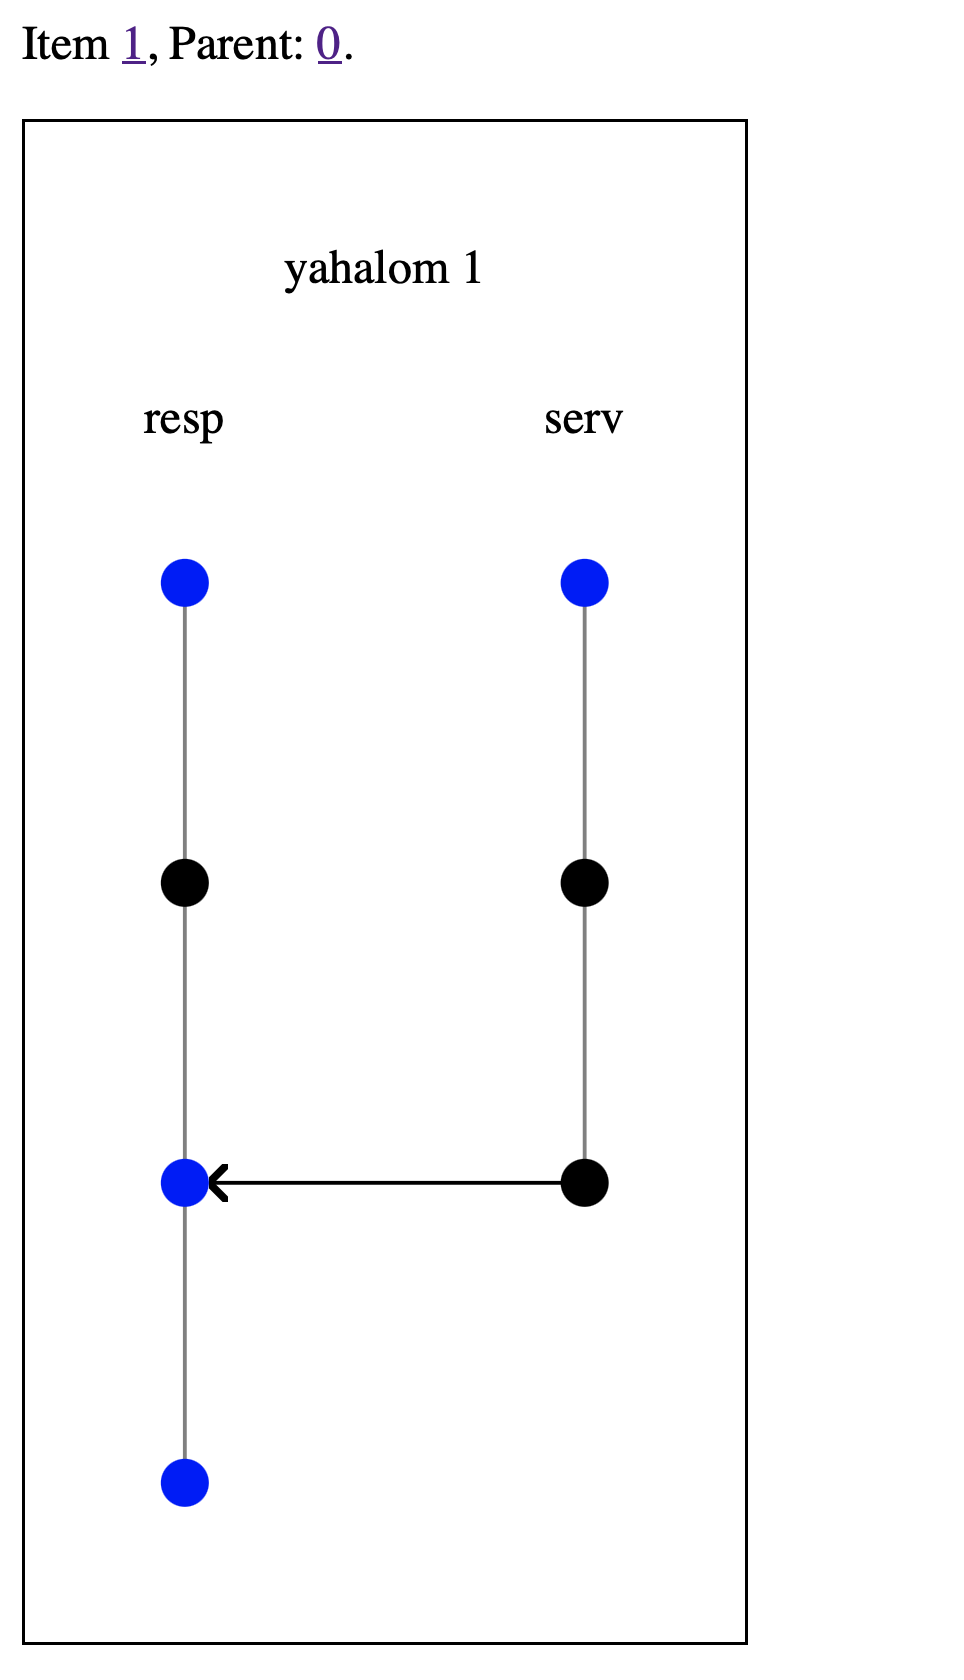
\includegraphics[height=2in]{yahalom_q_resp_pov1.png}
  \end{minipage}
  \begin{minipage}[c][2in][c]{.7\linewidth}\small
\begin{verbatim}(defskeleton yahalom
  (vars (k skey) (n-b n-a n-a-0 n-b-0 text)
                 (a b name) ...)
  (defstrand resp 4 (k k) (n-a n-a) (n-b n-b)
                    (b b) (a a) ...)
  (defstrand serv 3 (k k) (n-a n-a-0) (n-b n-b-0)
                    (a a) (b b) ...)
  (precedes ((1 2) (0 2)))
  (uniq-orig k n-b)
  (auth ch2) ...) \end{verbatim}
  \end{minipage}
  \caption{Responder's first guarantee}
  \label{fig:yahalom:q:resp:pov:1}
\end{figure}

Now that we have ascertained a server run occurred with the same
identities $A,B$ and session key $K$, we may resubmit this output to
{\cpsa} with the added annotation \texttt{(conf ch2 ch3)}, saying that
we will assume that \emph{this} server session successfully used
channels with the confidential property.  At this point, {\cpsa}
completes the analysis with the same shape shown in
Fig.~\ref{fig:yahalom:ch:resp:pov}.

This establishes that no other channel assumptions could be relevant
to the conclusion.  This was not evident from
Fig.~\ref{fig:yahalom:ch:resp:pov}, since other channel assumptions
may have led {\cpsa} to discard some branches of analysis as
impossible, which might then never be displayed.

The analysis from the initiator's point of view can then follow the
same pattern.  

\section{State}
\label{sec:channels:state:state}

{\cpsa} models situations in which regular principals control devices
with state registers or storage locations---we will henceforth use the
term \emph{location} for all such pieces of memory---that allow long
term storage and coordination among different local protocol sessions.%
%
\footnote{Allowing the Dolev-Yao adversary to have devices does not
  strengthen its powers, as it can already remember unbounded numbers
  of messages and perform all the reasonable operations on them.  This
  is why our model highlights devices under the control of the regular
  principals.}
%
Each protocol role determines when a regular principal reads from a
device location; what it does with the value read from it, and the
parts of the value; and when it writes a new value into a location.

\paragraph{Locations and channels.}  As we mentioned at the start of
the chapter, {\cpsa} relies on the analogy between reading from
locations and receiving messages from channels, and between writing to
locations and sending messages onto channels.  In particular, writing
to a location is like sending to a confidential channel, as we are
modeling regular principals in control of the devices.  And reading a
state value is partly like receiving from an authenticated channel:
Unless the value read might be the result of device initialization, it
must have been written by a previous write action by a regular
principal.  We say that a value is a \emph{generated state value} when
we model it as not a possible result of device initialization.  When
{\cpsa} knows of a value read from a location that it is a generated
state value, it treats this as an authenticated channel reception.  It
then investigates the possible ways that regular principals may
previously have written this state value to the location.

\paragraph{Contrast:  Locations are mutable.}  Channels can deliver
the same message more than once, and, since redelivery is never ruled
out, effectively always remember their previous contents.  However,
locations are mutable.  After a transition event observes the value in
a location and writes a new (possibly related) value into the
location, subsequent reads are guaranteed to deliver the new value,
not its predecessor.  Although any number of read events may observe
the same value, a transition event ensures that the new value is the
only value available from this location.  This fact---that transitions
erase the past---is the essential characteristic of mutable state.

\paragraph{``Leads to.''}  When a state transition event $n_0$ writes
a value $v$ into a state location $\ell$, and a later observation or
transition event $n_1$ obtains this value $v$ from $\ell$, without any
other transitions having occurred to $\ell$ in between, we say that
$n_0$ \emph{leads to} $n_1$, and we write $n_0\leadsto n_1$.

Thus, when $n_0\leadsto n_1$ the following conclusions hold:
\begin{renumerate}
  \item $n_0$ and $n_1$ are events on the same location $\ell$;
  \item  $n_0$ is a transition event;
  \item $n_0$ precedes $n_1$, also written $n_0\prec n_1$; and
  \item $n_1$ receives the value that $n_0$ has written into $\ell$.
\end{renumerate}
%
The event $n_1$ may just be a state observation rather than a state
transition.  In the former case, it is a pure read against $\ell$.  In
the latter case, it is the beginning of a transition event, which we
think of as consisting of a read of the old value in $\ell$ followed
by a write of the new value into $\ell$.

Internally, {\cpsa} represents a state event as transmitting or
receiving a pair $t=(p,v)$.  The second component is the state value
$v$ being read or written.  The first component is a special value
which is thought of as a spacetime point $p$.  If the event is a write
event, then {\cpsa} assumes $p$ to be uniquely originating.  {\cpsa}
defines $n_0\leadsto n_1$ to hold iff (i) $n_0$ is a state node; (ii)
$n_0\prec n_1$, and (iii) for some message $t$, $n_0$ transmits $t$
and $n_1$ receives $t$.

This {\cpsa} representation lets us add to (1)--(4) another
conclusion:  When $n_0\leadsto n_1$,
%
\begin{renumerate}
  \item if also $n_2\leadsto n_1$, then $n_0=n_2$.  
\end{renumerate}

\subsection{The axioms of state}
\label{sec:channels:state:axioms}

The mutating, past-erasing property of transitions is expressed in two
basic properties of the leads-to relation.  They say in essence that
leads-to is \emph{discrete} for transitions events on any one
location.

We write them diagrammatically in Fig.~\ref{fig:leads:to}, using a
boxed variable $\xymatrix@1{*+[F]{\,m\,\strut}}$ to represent a
transition event, and a plain variable $m$ to represent an event that
may be either a transition or a pure observation.  We use a wavy arrow
to represent leads-to; a dotted arrow to represent the precedence
ordering $\prec$; and $\preceq$ to express the weak ordering,
i.e.~$n_0\preceq n_1$ holds if and only if $n_0\prec n_1$ or
$n_0=n_1$.
%
\begin{figure}
  \centering
  %
  \[(i)\qquad
    \xymatrix@R=1mm@C=4mm{&
      *+[F]{n}\ar@{~>}[ddl]\ar@{.>}[ddr]^{\prec} & & & & 
      *+[F]{n}\ar@{~>}[ddl]\ar@{.>}[ddr]^{\prec} \\
      & & & \Longrightarrow &    \\
      *+[F]{m_0} & & *+[F]{m_1} & &
      *+[F]{m_0} & \textcolor{red}{\preceq} & *+[F]{m_1} } 
    %
  \]\vspace{3ex}
  %
  \[(ii)\qquad
    \xymatrix@R=1mm@C=4mm{*+[F]{m_0}\ar@{.>}[ddr]_{\prec} & &
      *+[F]{m_1}\ar@{~>}[ddl] & &
      *+[F]{m_0}\ar@{.>}[ddr]_{\prec} &\textcolor{red}{\preceq} &
      *+[F]{m_1}\ar@{~>}[ddl]\\
      & & & \Longrightarrow   \\
      & n && && n}    
  \]
  \caption[Leads-to axioms]{Two axioms about state events on the same
    location $\ell$}
  \label{fig:leads:to}
\end{figure}
%

In each case, the events $n,m_0,m_1$ are all state events on the same
location $\ell$.
%
\begin{description}
  \item[Axiom (i)] states that when $n\leadsto m_0$ and $n\prec m_1$,
  all of these being transition events on $\ell$, then
  $m_0\preceq m_1$.  Thus, the leads-to relation is a discrete step,
  and if $m_0\not= m_1$, then the latter comes definitely later.

  We call axiom (i) the \textbf{discrete-after} axiom, since it forces
  $m_1$ to come after a transition that is the target of the
  $\leadsto$ edge.
  \item[Axiom (ii)] states that when $m_0\prec n$ and $m_1\leadsto n$,
  each $m_i$ being a transition on $\ell$, then $m_0\preceq m_1$.
  Again, the leads-to relation is a discrete step, and if
  $m_0\not= m_1$, then the former comes definitely earlier.

  We call axiom (ii) the \textbf{discrete-before} axiom, since it
  forces $m_0$ to come before a transition that is the source of the
  $\leadsto$ edge.
\end{description}
%
The symmetry between these two principles is better brought out if we
omit to state, in (i), that $n$ is a transition.  The source of a
leads-to edge is always a transition.  The common idea is that a weak
ordering holds between $m_0$ and $m_1$, whenever one is a connected to
$n$ by $\leadsto$ and the other by $\prec$.  They jointly say:  a
transition ordered with respect to one end of a leads-to arrow has the
corresponding weak ordering with respect to the other end.

Their concrete form may be found in the output of {\cpsa}
specifications using state, such as~\texttt{examples/open-closed.tst},
although {\cpsa} refers to them as the \texttt{shearsRule} and
\texttt{invShearsRule}, resp.

\subsection{Consequences of the axioms}
\label{sec:channels:state:consequences}

What is distinctive of state---over and above channel confidentiality
and channel authenticity for generated state values---is captured in
the \emph{discrete-after} and \emph{discrete-before} axioms.  However,
each of them has a disjunction as its conclusion, namely either
$m_0=m_1$ or $m_0\prec m_1$.  Disjunctions are logically less
convenient than non-disjunctive conclusions, since separate
possibilities must each be explored.
%
\begin{figure}
  \centering\[ \xymatrix@R=1mm@C=1mm{&
      *+[F]{n}\ar@{~>}[ddl]\ar@{~>}[ddr] & \\
      & & & \Longrightarrow &  \textcolor{red}{m_0=m_1}  \\
      *+[F]{m_0} & & *+[F]{m_1}} \qquad\qquad
    %
    \xymatrix@R=1mm@C=1mm{&
      *+[F]{n_0}\ar@{~>}[ddl]\ar@{.>}[ddr]^{\prec} & \\
      & & & \Longrightarrow &  \textcolor{red}{\mathsf{false}}  \\
      *+[F]{n_1} &\succ & *+[F]{m}}
    %
  \]
  \[ \xymatrix@R=1mm@C=4mm{&
      *+[F]{n_0}\ar@{~>}[ddl]\ar@{~>}[ddr] & \\
      & & & \Longrightarrow &  \textcolor{red}{\mathsf{false}}  \\
      *+[F]{n_1} &\prec & {m}}
    % 
  \]  
  \caption{Three derived rules for state:  Scissors, no interruption,
    and cake}
  \label{fig:derived:state:rules}
\end{figure}
%
Hence, {\cpsa} also formalizes three consequences of the discreteness
axioms.  One of them has the conclusion $m_0=m_1$, and the other two
have the conclusion \emph {false}.  Again assuming that the state
events concern the same location $\ell$, the rules are:
%
\begin{description}
  \item[Scissors rule,] which says that when a given node $n$ leads to
  transition nodes $m_0,m_1$, the latter two are equal.

  Equivalently, a single node leads to at most one transition node.
  \item[No interruption,] which says that a transition node $m$ is
  never properly between transition nodes $n_0$ and $n_1$ when
  $n_0\leadsto n_1$.

  Thus, a transition node $m$ cannot ``interrupt'' the leads-to edge.
  \item[Cake rule,] which says that if a node $n_0$ leads to two other
  nodes, and one of them is a transition $n_1$, then the other one $m$
  does not follow the transition.

  Thus, it says that a transition $n_1$ caps off the period when other
  events $m$ (which are pure observations by the scissors rule) may
  result from $n_0$.  
\end{description}
%
We present these diagrammatically in
Fig.~\ref{fig:derived:state:rules}.  The two leads-to edges of the
\emph{scissors rule} are like the blades, which the equation
${m_0=m_1}$ snaps shut.  The cake rule formalizes the fact that you
can't eat your cake at $n_1$ and have it too at $m$, at least not if
$m$ follows $n_1$.

Again, their concrete form may be found in the output of {\cpsa}
specifications using state, such as~\texttt{examples/open-closed.tst}.

\paragraph{Why these rules are consequences.}  Each of these rules is
easily justified from the discrete-after and discrete-before rules,
using the facts that $n\leadsto m$ implies $n\prec m$ and that
$\preceq$ is a (weak) partial order.

\begin{description}
  \item[Scissors rule:]  The scissors rule follows by two applications
  of the discrete-after axiom.  Specifically, since $n\leadsto m_1$
  implies $n\prec m_1$, we can apply the discrete-after axiom to infer
  that $m_0\preceq m_1$.  Symmetrically, observing thay
  $n\leadsto m_0$ implies $n\prec m_0$, we can again apply the
  discrete-after axiom to infer that $m_1\preceq m_0$.

  The antisymmetry of $\preceq$ implies that $m_0=m_1$.
  \item[No interruptions rule:]  For the no interruptions rule, apply
  discrete-after to infer that $n_1\preceq m$.  But since
  $m \prec n_1$ is also assumed, this would yield a cycle.
  \item[Cake rule:]  For the cake rule, apply discrete-before,
  instantiating its variable $m_0$ as $m$, its $m_1$ as $n_0$, and its
  $n$ as $n_1$.  Thus, it follows that $m\preceq n_0$, but the
  leads-to edge $n_0\leadsto m$ implies $n_0\prec m$, yielding a
  contradiction.
\end{description}
   
\subsection{Syntax for state}
\label{sec:channels:state:syntax}

In defining the syntax for modeling state, we first describe state
events and the state segments that they can build up.  We then
describe how to specify generated state values---which were mentioned
at the beginning of the chapter---and critical sections---which are
atomicity assumptions about state segments.

\paragraph{State events and state segments.}  In addition to the
\verb|chan| sort discussed in Section~\ref{sec:channels:state:ch},
there is a sort \verb|locn|.  A variable \verb|lv| declared of sort
\verb|locn| via a declaration such as \verb|(lv locn)| may be used as
the target of \verb|load| and \verb|stor| events; these events
indicate that a value is to be read from a location or written to it.
Thus, Fig.~\ref{fig:dev:open}, which uses a number of operators from a
\texttt{lang} field,%
\footnote{See Section~\ref{sec:algebra:lang:field}.  In this example,
  \texttt{dev-key-state}, \texttt{open-req}, \texttt{door-state}, and
  \texttt{opened} are tuple operators, and \texttt{hash-dk} is a hash
  operator, in essence a key derivation function.  This example is
  found in~\texttt{examples/open-closed.scm}.}
%
shows a role that manipulates two variables \texttt{lk, ls} of sort
\verb|locn|.  Its intent is to open a door in response to a suitable
encrypted command, conforming its action.  
%
\begin{figure}\small
  % 
\begin{verbatim}(defrole dev-open
    (vars (k skey) (n nb text) (any mesg) (d o b name) (lk ls locn))
    (trace
     (load lk (dev-key-state d o k))
     (recv (cat b n (enc (open-req b d o nb n) (hash-dk (cat b nb n k)))))
     (load ls (door-state d any))
     (load lk (dev-key-state d o k))         ; check k unchanged 
     (stor ls (door-state d (opened b nb n)))
     (send (hash (open-req b d o nb n))))
    (gen-st (dev-key-state d o k))
    (facts (same-dev ls lk)))\end{verbatim}
  % 
  \caption{Device-open role causing door to open}
  \label{fig:dev:open}
\end{figure}
%
The form \texttt{(lk ls locn)} declares the variables of sort
\verb|locn|.  The form \texttt{(load lk (dev-key-state d o k))} loads
a tuple including a key \verb|k| from the \verb|locn| \verb|lk|, which
must contain a tuple of this kind for the event to occur.  After
receiving a message that contains a request to open the door, it loads
the current door state from the other location \verb|ls|, after which
it stores back the ``open'' value.  These events might be implemented
by a sensor and an actuator in a real device.  Finally, it confirms
success by sending the hash of the open request.

A \verb|load| or \verb|stor| event always contains a location variable
followed by a message term, just like a channel \verb|send| or
\verb|recv| (Section~\ref{sec:channels:state:ch}).

Observe that the \verb|stor| event immediately follows a \verb|load|
event, and this is in fact always the case.  Since together they
represent a transition that consumes an old value that will no longer
be available after the the transition, the \verb|stor| event always
follows a paired \verb|load| event.  Together, they form a \emph{state
  segment}.  However, state segments may be longer than a single pair
of events.

In general, a state segment consists of one or more \verb|load|
events followed by zero or more \verb|stor| events, subject to the
requirements that:
%
\begin{enumerate}
  \item no two \verb|load| events in this state segment load from the
  same location;
  \item no two \verb|stor| events in this state segment store into the
  same location;
  \item each \verb|stor| event stores into a location from which a
  value was \verb|load|ed in this state segment.
\end{enumerate}
%
A particular state segment is a \emph{transition for} a location
$\ell$ iff there is a \verb|stor| into $\ell$ in this state segment.
It is a \emph{(pure) observation for} $\ell$ iff there is a
\verb|load| from $\ell$ but no \verb|stor| into $\ell$ in this state
segment.

We use state segments of length greater than two to represent events
that involve multiple locations.  If a transition for location
$\ell_1$ depends on the value present in $\ell_2$, then a state
segment can load $v_1$ and $v_2$ from $\ell_1$ and $\ell_2$
(resp.)~and then store a new value dependent on $v_1,v_2$ into
$\ell_1$.  In this case, the state segment is a transition for
$\ell_1$ but a pure observation for $\ell_2$.  If instead new values
are stored into both $\ell_1$ and $\ell_2$, then the state segment is
a transition for both.  In other cases, a state segment loads from
both $\ell_1$ and $\ell_2$, but instead of storing back to either of
them, it simply uses those values to control future message
transmissions and receptions.  In the latter cases, the state segment
is a pure observation for both $\ell_1$ and $\ell_2$.  

\paragraph{Rules for protocols with
  state.}  \label{state:gen:rules:start} {\cpsa} generates three types
of rules for protocols that manipulate state, in addition to the two
axioms of Section~\ref{sec:channels:state:axioms} and the three
consequences of Section~\ref{sec:channels:state:consequences}.%
%
\footnote{See Section~\ref{sec: rules} for rules in {\cpsa}.}

The first kind are the \emph{transition rules}, and these are
generated entirely automatically by {\cpsa}.  The axioms and rules of
Sections~\ref{sec:channels:state:axioms}--\ref{sec:channels:state:consequences}
depend on which events are transition events, the boxed events in
Figs~\ref{fig:leads:to}--\ref{fig:derived:state:rules}.  Moreover, the
syntax of the state segments determines which these are.  Thus,
{\cpsa} generates rules that imply that an event is a transition event
if:
%
\begin{enumerate}
  \item it is a \verb|stor| event; or
  \item it is a \verb|load| event, and the strand is long enough also
  to have a \verb|stor| event from this state segment for the same
  location $\ell$.
\end{enumerate}
%
These are the transition rules.

The second kind are the \emph{generated state value rules}.  As we
mentioned at the start, a generated state value is a value $v$ that is
definitely non-initial.  Thus, if a \verb|load| event reads a
generated state value $v$ from a location $\ell$, then $\ell$ is
acting like an authenticated channel for $v$.  In particular {\cpsa}
will consider which instances of the roles could previously have
stored $v$ into $\ell$; one of those must be present.

A generated state assumption may be introduced as a per-strand
assumption, akin to the declarations discussed in
Section~\ref{sec:channels:state:ch:strand:level}.  In that case it is
syntactically present in a {\cpsa} \texttt{defskeleton} query such as:
%
{\small
\begin{verbatim}(defskeleton open-closed
  (vars (k skey) (d o name))
  (defstrand dev-pass 4 (k k) (d d) (o o))
  (gen-st (dev-key-state d o k)))
\end{verbatim}}
%
This \texttt{gen-st} declaration says that the particular tuple
\texttt{(dev-key-state d o k)} using the values of the variables that
appear in this strand forms a generated state value.

A generated state assumption may be introduced as a role-level
assumption, akin to the declarations discussed in
Section~\ref{sec:channels:state:ch:role:level}.  In this case, the
specifier wants to tell {\cpsa} that the declared value is a generated
state value whenever an instance of the role is long enough to furnish
values for the variables that appear in it.  Fig.~\ref{fig:dev:open}
contains a role-level generated state assumption, namely
\texttt{(dev-key-state d o k)}.  Since the trace of the
\texttt{dev-open} rule loads a value of this form as its first action,
these variables have values in every instance of height $\ge 1$.

{\cpsa} enforces this role-level assumption by generating a rule
stating:
%
{\small
\begin{verbatim}(defgenrule gen-st-dev-open-0
    (forall ((z strd) (k skey) (o d name))
      (implies
        (and (p "dev-open" z 1) (p "dev-open" "k" z k)
             (p "dev-open" "o" z o) (p "dev-open" "d" z d))
        (gen-st (dev-key-state d o k)))))
\end{verbatim}
}
%
\noindent{\cpsa} uses the \texttt{defgenrule} form to distinguish
rules it has generated automatically from rules that were explicitly
written by the specifier, as described in Section~\ref{sec: rules}.

Finally, the third kind of rule concerns \emph{critical sections}.
%
\begin{figure}\small
%
\begin{verbatim}(defrole dev-up
    (vars (k skey) (d o name) (old old1 mesg) (ch chan) (lk ls locn))
    (trace
     (recv ch (cat "power-up" d o k))
     (load lk old)
     (load ls old1)
     (stor lk (dev-key-state d o k))
     (stor ls (door-state d (closed o)))
     (send (enc "up" k)))
    (auth ch)
    (critical-sections (1 4))
    (facts (same-dev ls lk)))
\end{verbatim}
%
  \caption{Critical section declaration}
  \label{fig:critical:section}
\end{figure}
%
%
\begin{figure}\small
  % 
\begin{verbatim}  (defgenrule cau-dev-up-2
    (forall ((z z1 strd) (i indx))
      (implies
        (and (p "dev-up" z 3) (prec z1 i z 2))
        (or (= z z1) (prec z1 i z 1)))))

  (defgenrule eff-dev-up-3
    (forall ((z z1 strd) (i indx))
      (implies 
        (and (p "dev-up" z 4) (prec z 3 z1 i))
        (or (= z z1) (and (p "dev-up" z 5) (prec z 4 z1 i))))))\end{verbatim}
%  
  \caption{Critical section:  Generated rules}
  \label{fig:critical:section:rules}
\end{figure}
%
A critical section declaration in the definition of a role takes the
form \texttt{(critical-sections (i j))}, where the trace must have a
state segment that starts at or before event \emph{i} and ends at or
after event $j$, where these are 0-based indices.  It implies that any
node that precedes one of the load events must precede all of them.
Any node that follows one of the store events must follow all of them.
Thus for instance in Fig.~\ref{fig:critical:section}, the load events
at indices 1, 2 and the store events at indices 3, 4 occur with
transaction-like atomicity.  This declaration would cause {\cpsa} to
generate the rules in Fig.~\ref{fig:critical:section:rules}.  They are
of value only when the state segment has multiple loads or multiple
stores.  In this particular example, the critical section declaration
does not in fact make a difference to the analysis.
%
\label{state:gen:rules:end}

\subsection{Channels and state:  Summary}
\label{sec:channels:state:summary}

A core idea is that receptions may have \emph{authenticity}, meaning
that the adversary has not delivered the message; thus, {\cpsa}
explores what regular strands may have transmitted it.  Dually, a
transmission may have \emph{confidentiality}, meaning that the
adversary will not receive the message directly.  Thus, any parts of
the transmitted message that appear in new forms subsequently will
require some regular strand to have received it and transformed these
parts.

In the {channel} mechanism, {\cpsa} allows these properties to be
directly associated with channels, providing a useful technique for
protocol design.  In the state mechanism, {\cpsa} models the
\emph{confidentiality} of storing a value into a device controlled
locally by the regular principal(s).  Moreover, \emph{stored} state
values with the \texttt{gen-st} property satisfy the
\emph{authenticity} condition also.

Besides these properties, mutable state also requires modeling the
fact that an old state value can no longer be observed in a location
after that location has undergone a transition.  We express these in
the two axioms of Fig.~\ref{fig:leads:to}; {\cpsa} also uses their
three consequences as shown in Fig.~\ref{fig:derived:state:rules} for
efficiency.

The modeling distinguishes between \emph{transitions} on a location,
which are expressed in state segments that contain a \verb|stor| to
it, and \emph{observations}, expressed in state segments that contain
a \verb|load| but no \verb|stor| to it.  {\cpsa} determines which
events are transitions on a location automatically, and generates
rules to keep track of this information.  Rules are also available to
determine which state values are \emph{stored} state values, and these
are generated from \texttt{gen-st} declarations.

{\cpsa}'s job is to enumerate shapes.  When a specification
distinguishes a kind of value that can only appear in an initial
\verb|load|, and transitions that do not produce these values, but
always produce \emph{stored} state values with the \texttt{gen-st}
property, then a run can typically have 0, 1, 2, \dots, $n$
transitions, and these will have no homomorphisms between them.  Hence
there will be infinitely many distinct shapes to enumerate, and
{\cpsa} will not terminate, although its partial outputs are often
informative.  The craft of using {\cpsa} to understand state in
protocols is often to restrict the \texttt{gen-st} declarations so
that {\cpsa} does not distinguish among state histories of
(irrelevantly) different lengths.


%%% Local Variables:
%%% mode: latex
%%% TeX-master: "cpsa4manual"
%%% End:
